
\subsubsection{Problemas GRPC en golang e interfaces de usuario}\label{subsubsec:problemas-rpc-en-golang}

Al enfrentar el desarrollo de un frontal, \textit{frontend}, para la interacción del usuario con el programa Manager se enfrentó el problema del estado del arte en dos puntos:
\begin{itemize}
    \item El uso de Go para realizar interfaces web de usuario se encuentra en un estado experimental.
    Habría supuesto más investigación de la proyectada
    \item GRPC en los navegadores web todavía no es compatible para todos los métodos de comunicación (Apartado ~\ref{GRPCcompatibilidadConNavegadores}).
\end{itemize}

El lenguaje utilizado es Typescript con el \textit{framework} React.
La decisión fue tomada por la facilidad de implementación de forma rápida y eficiente.
Se dispone de conocimiento previo con la herramienta.

En la ejecución manual de tareas el caso de uso para su uso en la interfaz de usuario tuvo que ser modificado.
Con el objetivo de visualizar en tiempo real la gráfica de los resultados obtenidos durante la ejecución de la tarea.
Inicialmente el diseño contemplaba explotar la opción del stream bidireccional para poder enviar los \textit{Steps} a requerimiento del usuario y obtener la respuestas en paralelo como se muestra en el diagrama UML de secuencia~\cref{fig:1-ExecuteTaskManuallyInteractionOriginal}.
Al no disponer del stream bidireccional se ha rediseñado un flujo alternativo.
El flujo original se encuentra descrito en el apartado~\ref{ref:X} describe el TaskLoop~\cref{fig:Use Case-TaskLoop} y el task Processor~\cref{fig:Use Case-Task Processor}.
El looper no ha tenido que sufrir modificaciones, demostrando que la arquitectura protege del cambio, pero el procesador para las tareas manuales ha sido desarrollado en otro servicio, haciendo uso del concepto de responsabilidad única o \textit{Open Close};
abierto a la extension, cerrado al cambio.

Los efectos en el Dominio son:
\begin{itemize}
    \item Las tareas bidireccionales son forzadas a contener como máximo 2 steps: una de comienzo y otra de fin.
    \item Se ha rediseñado el flujo bidireccional.
    El nuevo diseño consta de un proceso en el que se envía el primer step y se queda en un loop infinito.
    El proceso se encuentra a la escucha del cambio manual del estado de la tarea.
    Sólo una acción paralela que ejecute el cambio manual, mediante la edición de la Task a través de la llamada correspondiente, del status a DONE\@.
\end{itemize}

y los nuevos flujos diseñados se muestran en la~\cref{fig:1-ExecuteTaskManuallyInteractionV2} y la ~\cref{fig:1-TaskProcessorV2}.
Los cambios sufridos en la instanciación de la \textit{Task} se muestran en el~\cref{lst:Task}

\begin{figure}[H]
    \centering
    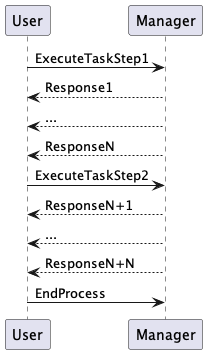
\includegraphics[height=0.4\textheight]{./part/Ejecucion/Seguimiento/MemoriaExplicativaDeCambios/img/1-ExecuteTaskManuallyInteractionOriginal}
    \caption{Use Case: 1-ExecuteTaskManuallyInteraction V2}\label{fig:1-ExecuteTaskManuallyInteractionOriginal}
\end{figure}
\begin{figure}[H]
    \centering
    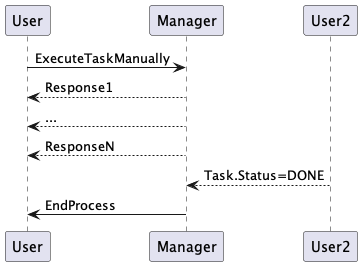
\includegraphics[height=0.3\textheight]{./part/Ejecucion/Seguimiento/MemoriaExplicativaDeCambios/img/1-ExecuteTaskManuallyInteraction}
    \caption{Use Case: 1-ExecuteTaskManuallyInteraction V2}\label{fig:1-ExecuteTaskManuallyInteractionV2}
\end{figure}

\begin{figure}[H]
    \centering
    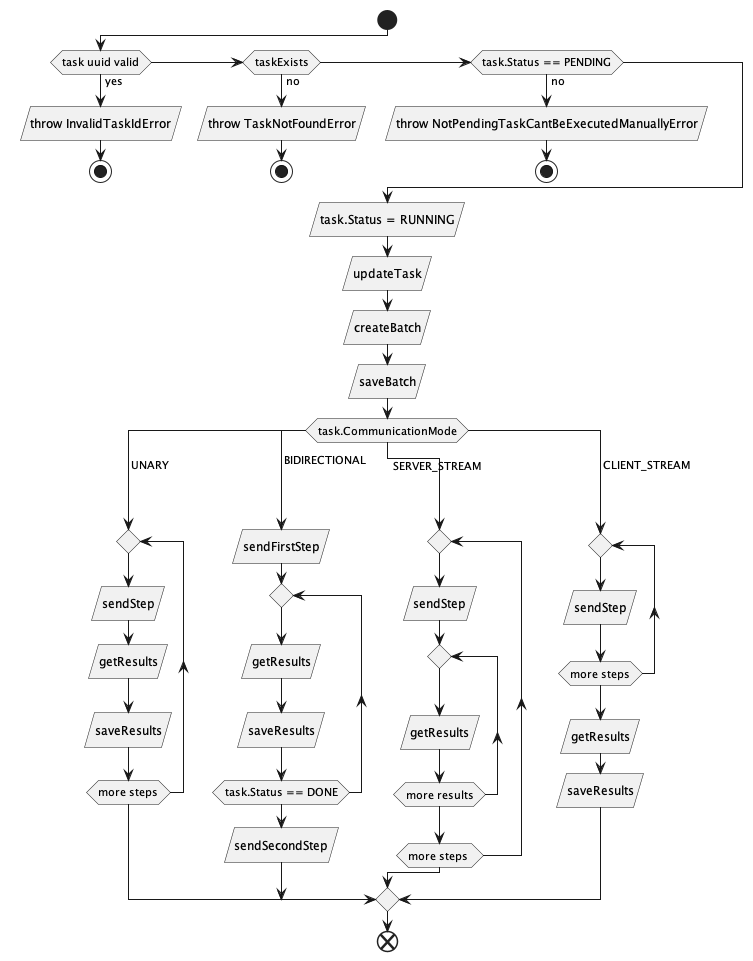
\includegraphics[height=0.7\textheight]{./part/Ejecucion/Seguimiento/MemoriaExplicativaDeCambios/img/1-TaskProcessor}
    \caption{Use Case: 1-TaskProcessor V2}\label{fig:1-TaskProcessorV2}
\end{figure}



\phantom{blank}
\vspace{5mm}
\hrule
\begin{lstlisting}[language=Go,caption={Clase Task.go Modificación},breaklines=true,label={lst:Task}]
package Task

import (
	"github.com/Enrikerf/pfm/commandManager/app/Domain/Task/CommunicationMode"
	"github.com/Enrikerf/pfm/commandManager/app/Domain/Task/Error"
	"github.com/Enrikerf/pfm/commandManager/app/Domain/Task/ExecutionMode"
	"github.com/Enrikerf/pfm/commandManager/app/Domain/Task/Host"
	"github.com/Enrikerf/pfm/commandManager/app/Domain/Task/Port"
	"github.com/Enrikerf/pfm/commandManager/app/Domain/Task/Status"
	"github.com/Enrikerf/pfm/commandManager/app/Domain/Task/Step"
)

type Task interface {
	GetId() Id
	GetHost() Host.Vo
	GetPort() Port.Vo
	GetSteps() []Step.Step
	GetCommunicationMode() CommunicationMode.Mode
	GetExecutionMode() ExecutionMode.Mode
	GetStatus() Status.Status
	SetHost(host Host.Vo)
	SetPort(port Port.Vo)
	SetStatus(status Status.Status)
}

type task struct {
	id                Id
	host              Host.Vo
	port              Port.Vo
	steps             []Step.Step
	communicationMode CommunicationMode.Mode
	executionMode     ExecutionMode.Mode
	status            Status.Status
}

func New(
	host Host.Vo,
	port Port.Vo,
	stepVos []Step.Vo,
	communicationMode CommunicationMode.Mode,
	executionMode ExecutionMode.Mode,
) (Task, error) {
	err := validateInputs(stepVos, communicationMode, executionMode)
	if err != nil {
		return nil, err
	}
	task := &task{}
	task.id = NewId()
	for _, stepVo := range stepVos {
		step := Step.New(stepVo)
		task.steps = append(task.steps, step)
	}
	task.host = host
	task.port = port
	task.executionMode = executionMode
	task.communicationMode = communicationMode
	task.status = Status.New(Status.Pending)
	return task, nil
}
func validateInputs(
	stepVos []Step.Vo,
	communicationMode CommunicationMode.Mode,
	executionMode ExecutionMode.Mode) error {
	<@\textcolor{red}{validación de consistencia de la definición de la Task}@>
	if len(stepVos) < 1 {
		return Error.NewTaskMustHaveAtLeastOneStepError()
	}
	if (communicationMode == CommunicationMode.Unary || communicationMode == CommunicationMode.ServerStream) &&
		len(stepVos) > 1 {
		return Error.NewCommunicationModeCanOnlyHaveOneStepError()
	}
	if executionMode == ExecutionMode.Manual && communicationMode == CommunicationMode.Bidirectional &&
		len(stepVos) > 2 {
		return Error.NewManualBidirectionalTaskOnlyCanHave2StepsError()
	}
	return nil
}

//... (Getters and Setters)


\end{lstlisting}
\hrule

\subsubsection{Caso práctico de las ventajas del \textit{DDD} y arquitectura de capas}

En el proceso de desarrollo se evaluó el coste de separar el programa ejecutado por parte del cliente y el cliente, conforme al diseño original.
Requería de una nueva implementación de intercomunicación que añadía complejidad y tiempo.
Al ser un proyecto amplio y abordar todo el proceso de desarrollo no consideró interesante esa complejidad añadida.
Por lo tanto, se introdujo la lógica del programa de control dentro del programa cliente.
Esta decisión permite ver la utilidad de la arquitectura al no encontrar ninguna fricción en este proceso.
Dos programas con el mismo diseño estructural y organización para unirse o separarse sólo requiere mover archivos y requiere desarrollo añadido.

El dominio se une sin afectarse el uno al otro ya que son independientes todos los elementos.
En la aplicación son casos de uso nuevos que tampoco interaccionan unos con otros.
y la infraestructura es totalmente diferente para cada programa y tampoco se afectan entre sí.
Se muestra en la~\cref{fig:Client+Control-Estructura de carpetas de Dominio},
~\cref{fig:Client+Control-Estructura de carpetas de Aplicación}
~\cref{fig:Client+Control-Estructura de carpetas de Infraestructura}
Que la estructura de carpetas es simplemente la suma de ambas estructuras.
El único punto de integración es que en los casos de uso de \textit{Step} (\textit{ExecuteUnary}, \textit{ExecuteServerStream}, \textit{ExecuteClientStream},\textit{ExecuteBidirectional}) se hace uso directo de los casos de uso del \textit{Engine}.
Es decir, que unos casos de uso de aplicación sirven como \textit{proxy} para los otros.

En el proyecto constará de 4 carpetas principales

\tiny
\dirtree{%
    .1 Project .
        .2 Domain.
        .2 Application.
        .2 Adapter.
        .2 Bootstrap.
}
\normalsize

\textbf{Dominio}

\begin{figure}[H]
    \tiny
\dirtree{%
    .1 Domain.
        .2 Step.
            .3 StepVo.
            .3 Repository.
                .4 consoleWrite.
            .3 Services.
                .4 Executor.
        .2 Result.
            .3 ResultVo.
}
\normalsize
    \caption[Diagrama de objetos de dominio]{}\label{fig:1-ClientDomainFolderStructure}
\end{figure}

\textbf{Aplicación}

\tiny
\dirtree{%
.1 Application.
    .2 Port.
        .3 in.
            .4 Step.
                .5 Execute.
                    .6 Command.
                    .6 UseCase.
}
\normalsize

\textbf{Adapters}

\tiny
\dirtree{%
    .1 Adapter.
        .2 in.
            .3 GRPC.
                .4 Harán uso de los useCases de aplicación cuando llegue una request RPC.
            .3 Console.
                .4 Por ejemplo si quisieramos ejecutar los casos de uso mediante terminal.
        .2 out.
            .3 console.
                .4 implementación de los repository de llamada a los servidores clientes.
}
\normalsize